\section{Analysis method}
\label{Sec:Analysis method}
In this article the \pT-differential non-linear flow modes are calculated  according to Eqs. \ref{Eq:VA422}-\ref{Eq:VA6222} with a method explained in \cite{Bilandzic:2013kga}. Each event is divided into two subevents ``$\rm{A}$'' and ``$\rm{B}$'', covering the ranges $-0.8< \eta < 0.0$ and $0.0 <\eta< 0.8$, respectively. Thus $v_{n,mk}(p_{\rm{T}})$ is a weighted average of $v_{n,mk}^{\rm{A}}(p_{\rm{T}})$ and $v_{n,mk}^{\rm{B}}(p_{\rm{T}})$. The measured $v_{n,mk}^{\rm{A}} (v_{n,mk}^{\rm{B}})$ coefficients are calculated using $d^{\rm{A(B)}}_{n,mk}(p_{\rm{T}})$ and $c_{mkmk}$ multi-particle correlators. In this analysis, $d^{\rm{A(B)}}_{n,mk}(p_{\rm{T}})$ is measured by selecting the identified hadrons (POIs) from subevent ``$\rm{A}$''(``$\rm{B}$'') and the reference particles from subevent ``$\rm{B}$''(``$\rm{A}$'') and $c_{mkmk}$ by selecting half of the reference particles from subevent ``$\rm{A}$'' and the other half from ``$\rm{B}$''. Thus, Eqs.\ref{Eq:V422} to \ref{Eq:V6222} for $v_{n,mk}^{\rm{A}}(p_{\rm{T}})$ translate to

\begin{align}
v_{4,22}^{\rm{A}}(p_{\rm{T}}) &= \frac{d_{4,22}^{\rm{A}}(p_{\rm{T}})}{\sqrt{c_{2222}}} =  \frac{\langle\langle \cos(4\varphi^{\rm{A}}_{1}(p_{\rm{T}})-2\varphi^{\rm{B}}_{2}-2\varphi^{\rm{B}}_{3})\rangle\rangle}{\sqrt{\langle\langle \cos(2\varphi^{\rm{A}}_{1}+2\varphi^{\rm{A}}_{2}-2\varphi^{\rm{B}}_{3}-2\varphi^{\rm{B}}_{4}) \rangle\rangle}}, \label{Eq:VA422} \\
v_{5,32}^{\rm{A}}(p_{\rm{T}}) &= \frac{d_{5,32}^{\rm{A}}(p_{\rm{T}})}{\sqrt{c_{3232}}} = \frac{\langle\langle \cos(5\phi^{\rm{A}}_{1}(p_{\rm{T}})-3\varphi^{\rm{B}}_{3}-2\varphi^{\rm{B}}_{2})\rangle\rangle}{\sqrt{\langle\langle \cos(3\varphi^{\rm{A}}_{1}+2\varphi^{\rm{A}}_{2}-3\varphi^{\rm{B}}_{3}-2\varphi^{\rm{B}}_{4}) \rangle\rangle}}, \label{Eq:VA532}\\
v_{6,33}^{\rm{A}}(p_{\rm{T}}) &= \frac{d_{6,33}^{\rm{A}}(p_{\rm{T}})}{\sqrt{c_{3333}}} =\frac{\langle\langle \cos(6\varphi^{A}_{1}(p_{\rm{T}})-3\varphi^{\rm{B}}_{2}-3\varphi^{\rm{B}}_{3})\rangle\rangle}{\sqrt{\langle\langle \cos(3\varphi^{\rm{A}}_{1}+3\varphi^{\rm{A}}_{2}-3\varphi^{\rm{B}}_{3}-3\varphi^{\rm{B}}_{4}) \rangle\rangle}}, \label{Eq:VA633}\\
v_{6,222}^{\rm{A}}(p_{\rm{T}}) &= \frac{d_{6,222}^{\rm{A}}(p_{\rm{T}})}{\sqrt{c_{222222}}} =\frac{\langle\langle \cos(6\varphi^{\rm{A}}_{1}(p_{\rm{T}})-2\varphi^{\rm{B}}_{2}-2\varphi^{\rm{B}}_{3}-2\varphi^{\rm{B}}_{4})\rangle\rangle}{\sqrt{\langle\langle \cos(2\varphi^{\rm{A}}_{1}+2\varphi^{\rm{A}}_{2}+2\varphi^{\rm{A}}_{3}-2\varphi^{\rm{B}}_{4}-2\varphi^{\rm{B}}_{5}-2\varphi^{\rm{B}}_{6}) \rangle\rangle}},
\label{Eq:VA6222}
\end{align}

%where $d^{\rm{A}}_{n,-m,-k}(p_{\rm{T}})$ and $c_{m,k,-m,-k}$ are each multi-particle correlations calculated with 2 subevent method generic framework. Details of this technique can be found in \cite{Bilandzic:2013kga}. 
where $\langle\langle\rangle\rangle$ denotes an average over all particles and events.
%The final measured $v_{n,mk}$ coefficients are calculated as a weighted average of $v_{n,mk}^{\rm{A}}$ and $v_{n,mk}^{\rm{B}}$ with the inverse of the square of the statistical uncertainty being the weight.

%The $v_{n,mk}(p_{\rm{T}})$ of the \Ks, \lambdas~and $\phi$ meson cannot directly be measured using Eq. \ref{Eq:VA422}-\ref{Eq:VA6222} as they cannot be identified on a particle-by-particle basis.

For inclusive charged hadrons, i.e. \pion, \kaon~and \proton, the $d_{n,mk}$ correlators are calculated on a track-by-track basis as a function of \pT~per centrality percentile. 

For particle species reconstructed on statistical basis from decay products, i.e. \Ks, \lambdas~and $\phi$ meson, the selected sample contains both signal and the combinatorial background. Therefore, for the aforementioned particle species, the $d_{n,mk}$ correlators are measured as a function of invariant mass (${\rm M_{inv}}$)~and \pT~per centrality percentile. The $d_{n,mk}$ vs. \minv~method is based on the additivity of correlations and is a weighted sum of the $d_{n,mk}^{\rm{sig}}$ and $d_{n,mk}^{\rm{bkg}}$ according to

\begin{equation}
d_{n,mk}({\rm M}_{\rm inv}) = \frac{N^{\rm sig}}{N^{\rm sig}+N^{\rm bkg}}({\rm M}_{\rm inv})d_{n,-m,-k}^{\rm sig}+\frac{N^{\rm bkg}}{N^{{\rm sig}}+N^{{\rm bkg}}}({\rm M}_{\rm inv})d_{n,-m,-k}^{\rm bkg}({\rm M}_{\rm inv}),
\label{Eq:dnmk}
\end{equation}

where $N^{\rm{sig}}$ and $N^{\rm{bkg}}$ are signal and background yields obtained for each \pT~interval and centrality percentile from fits to \Ks, \lambdas~and $\phi$ meson invariant mass distributions.% described in \ref{SubSec:K0sLambdaRec} and \ref{SubSec:PhiRec}. 
To obtain the \pT-differential yield of \Ks~and \lambdas~(which, together with background yields), are used for the signal extraction in Eq. \ref{Eq:dnmk}, invariant mass distributions at various \pT~intervals are parametrized as a sum of two Gaussian distribution and a third-order polynomial function. The latter is introduced to account for residual contamination (background yield) that are present in the \Ks~and \lambdas~signals after the topological and daughter track selections. The \Ks~and \lambdas~yields are extracted by integration of the Gaussian distribution. %The v_{n,mk}(\pT) results are reported for 1 < \pT < 6 GeV/c for \Ks and 1 < \pT < 6 GeV/c for \lambdas.
Similarly, to obtain the \pT-differential yield of $\phi$-mesons, the invariant mass distributions of the candidate yield is parametrized as a sum of a Breit-Wigner distribution and a third-order polynomial function, the latter introduced to account for residual contamination.

To extract $d_{n,mk}^{\rm{sig}}$, $d_{n,mk}({\rm M_{inv}})$ is fitted together with the fit values from the invariant mass distribution and parametrising $d_{n,mk}^{\rm{bkg}}({\rm M_{inv}})$ with a first order polynomial function. Figure \ref{d422_phi_meson} illustrates this procedure for the $\phi$-meson, with the invariant mass distribution in the upper panel and the measurement of $d_{4,22}({\rm M_{inv}})$ in the lower panel. 

\begin{figure}[!htb]
\begin{center}
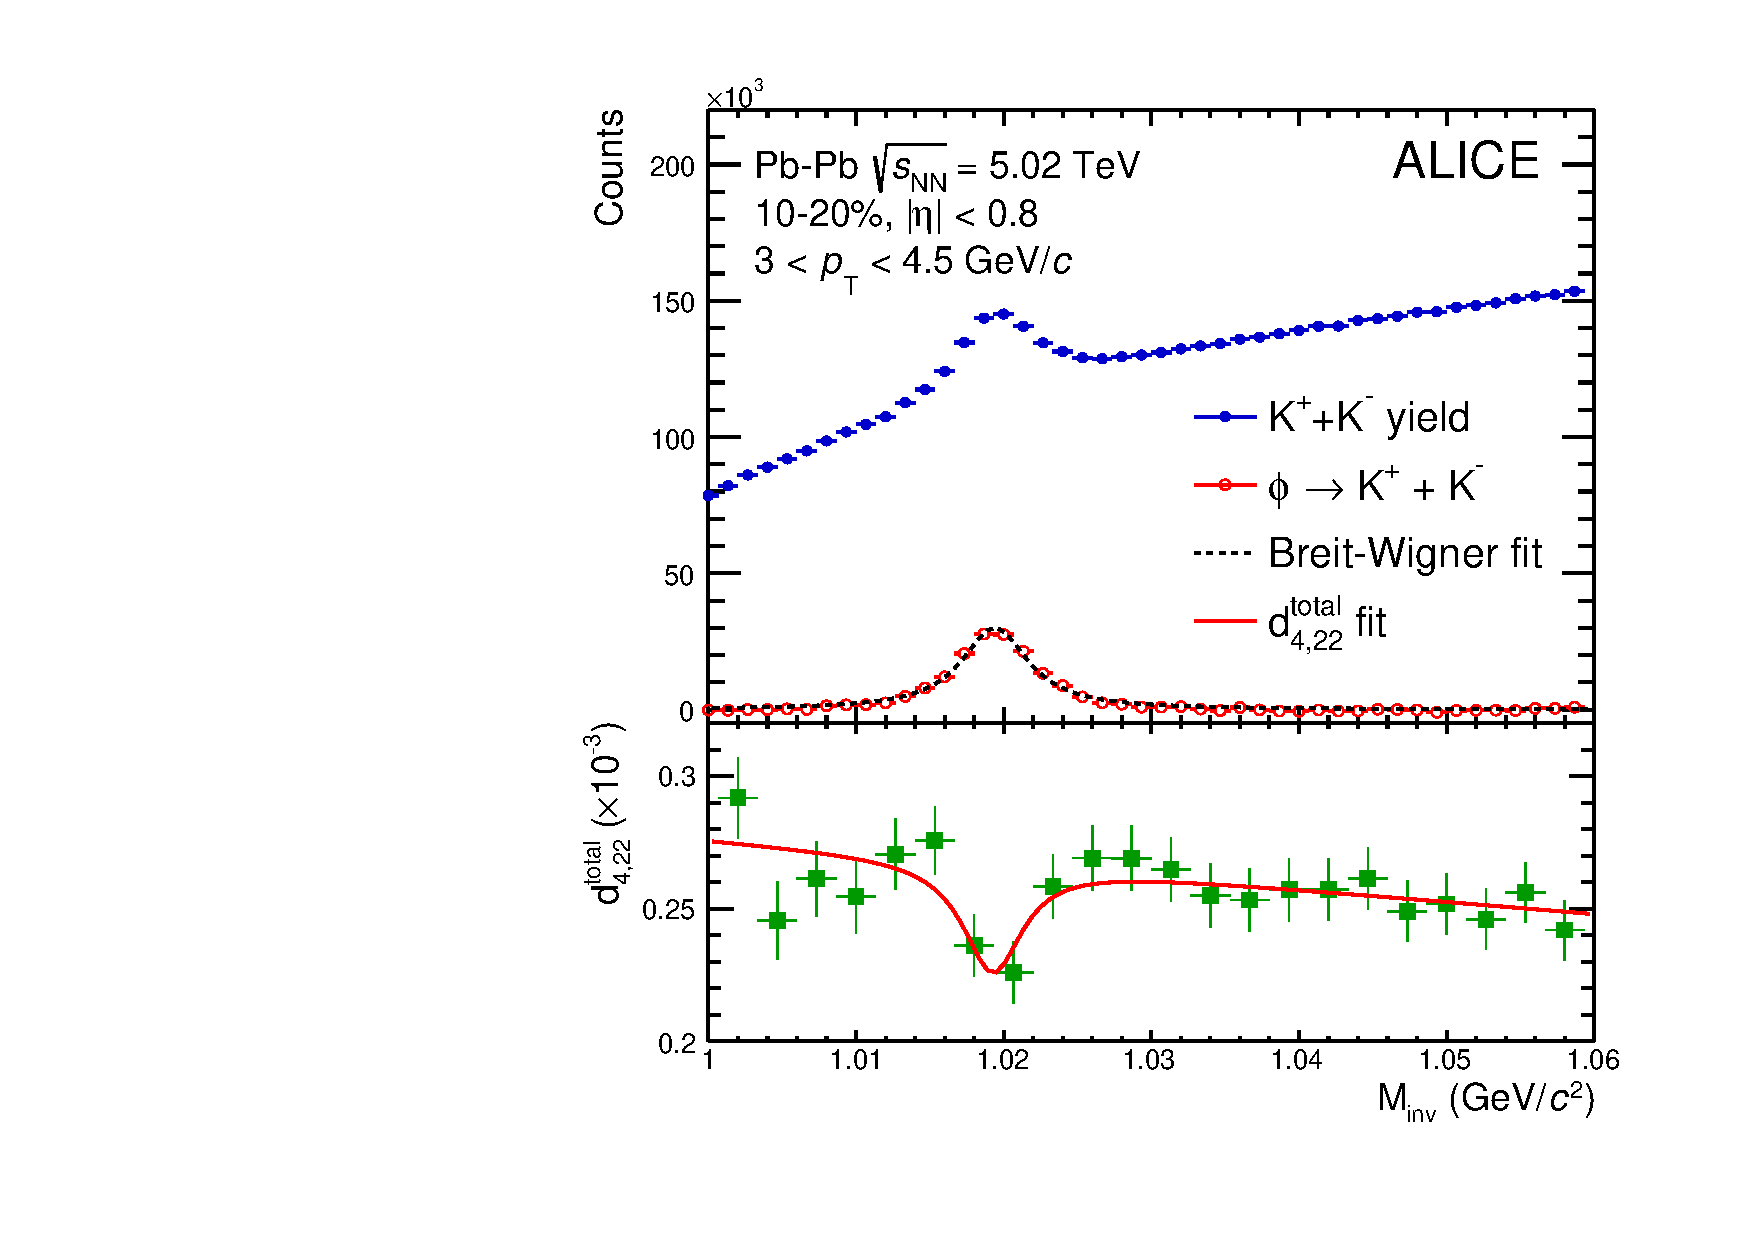
\includegraphics[scale=0.45]{figures/analysisMethod/flowmass_Phi.pdf}
\end{center}
\caption{Reconstruction and $d_{4,22}$ measurement of $\phi$-meson. Upper panel: extraction of $N^{\rm{sig}}$ and $N^{\rm{bkg}}$ by fitting the invariant mass ($m_{\rm{inv}}$) distribution for $\phi$-meson for $3<p_{\rm{T}}<4.5~{\rm GeV}/c$ at 10-20\% centrality interval, lower panel: extraction of $d_{4,22}^{sig}$ by fitting Eq. \ref{Eq:dnmk} to the invariant mass dependence of $d_{4,22}$}
\label{d422_phi_meson}
\end{figure}


%To estimate the signal and background yields, the invariant mass distributions of selected candidates are fitted with sum of the signal and background yields. 